\documentclass[french]{beamer}

\usepackage[utf8]{inputenc}
\usepackage[T1]{fontenc}
\usepackage{lmodern}
\usepackage{amsmath, amssymb}

\usepackage{babel}


%CHOIX DU THEME et/ou DE SA COULEUR
% => essayer différents thèmes (en décommantant une des trois lignes suivantes)
\usetheme{PaloAlto}
%\usetheme{Madrid}
%\usetheme{Copenhagen}

% => il est possible, pour un thème donné, de modifier seulement la couleur
%\usecolortheme{crane}
%\usecolortheme{seahorse}

%\useoutertheme[left]{sidebar}


%Pour le TITLEPAGE
\title{Projet de Recherche}
\author[]{TOULLALAN Antoine MENDAS Rosa}
\date{Lundi 1er Mars (7e réunion)}
\begin{document}
 \section{LeafSet d'un réseau de Pastry}
\begin{frame}{LeafSet d'un réseau de Pastry}
\begin{Large}
On suppose qu'on a un réseau de Pastry avec un LeafSet L de taille |L|, C est un noeud dont le nodeID est contenu à la case i de L, on note cette case Li.
\end{Large}
 \end{frame}
 \begin{frame}{LeafSet d'un réseau de Pastry}
 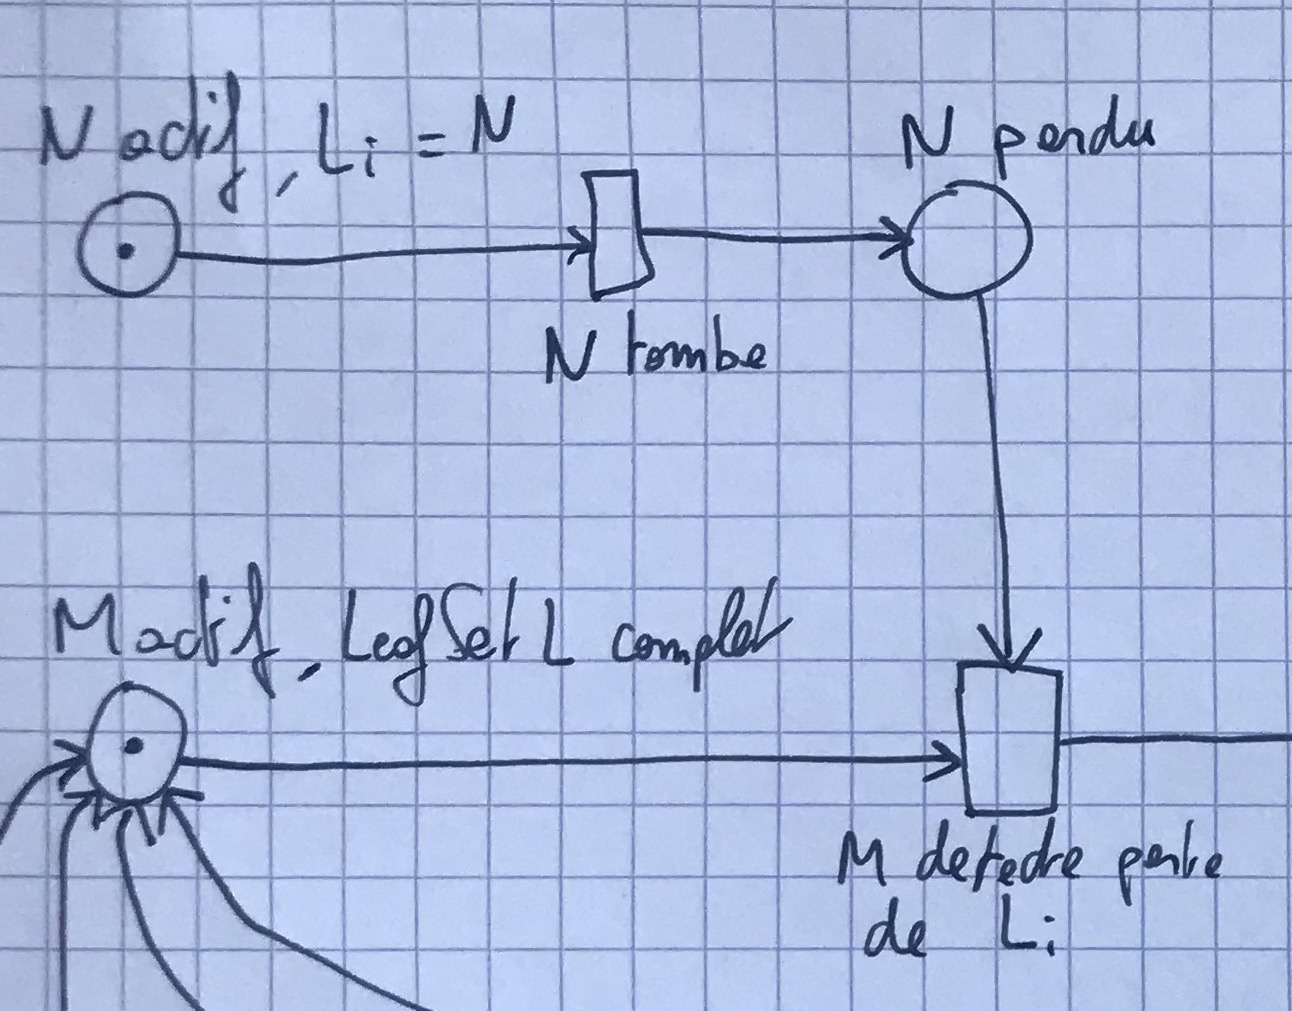
\includegraphics[scale=0.2]{partie1.jpg}
 \end{frame}
 \begin{frame}{LeafSet d'un réseau de Pastry}
 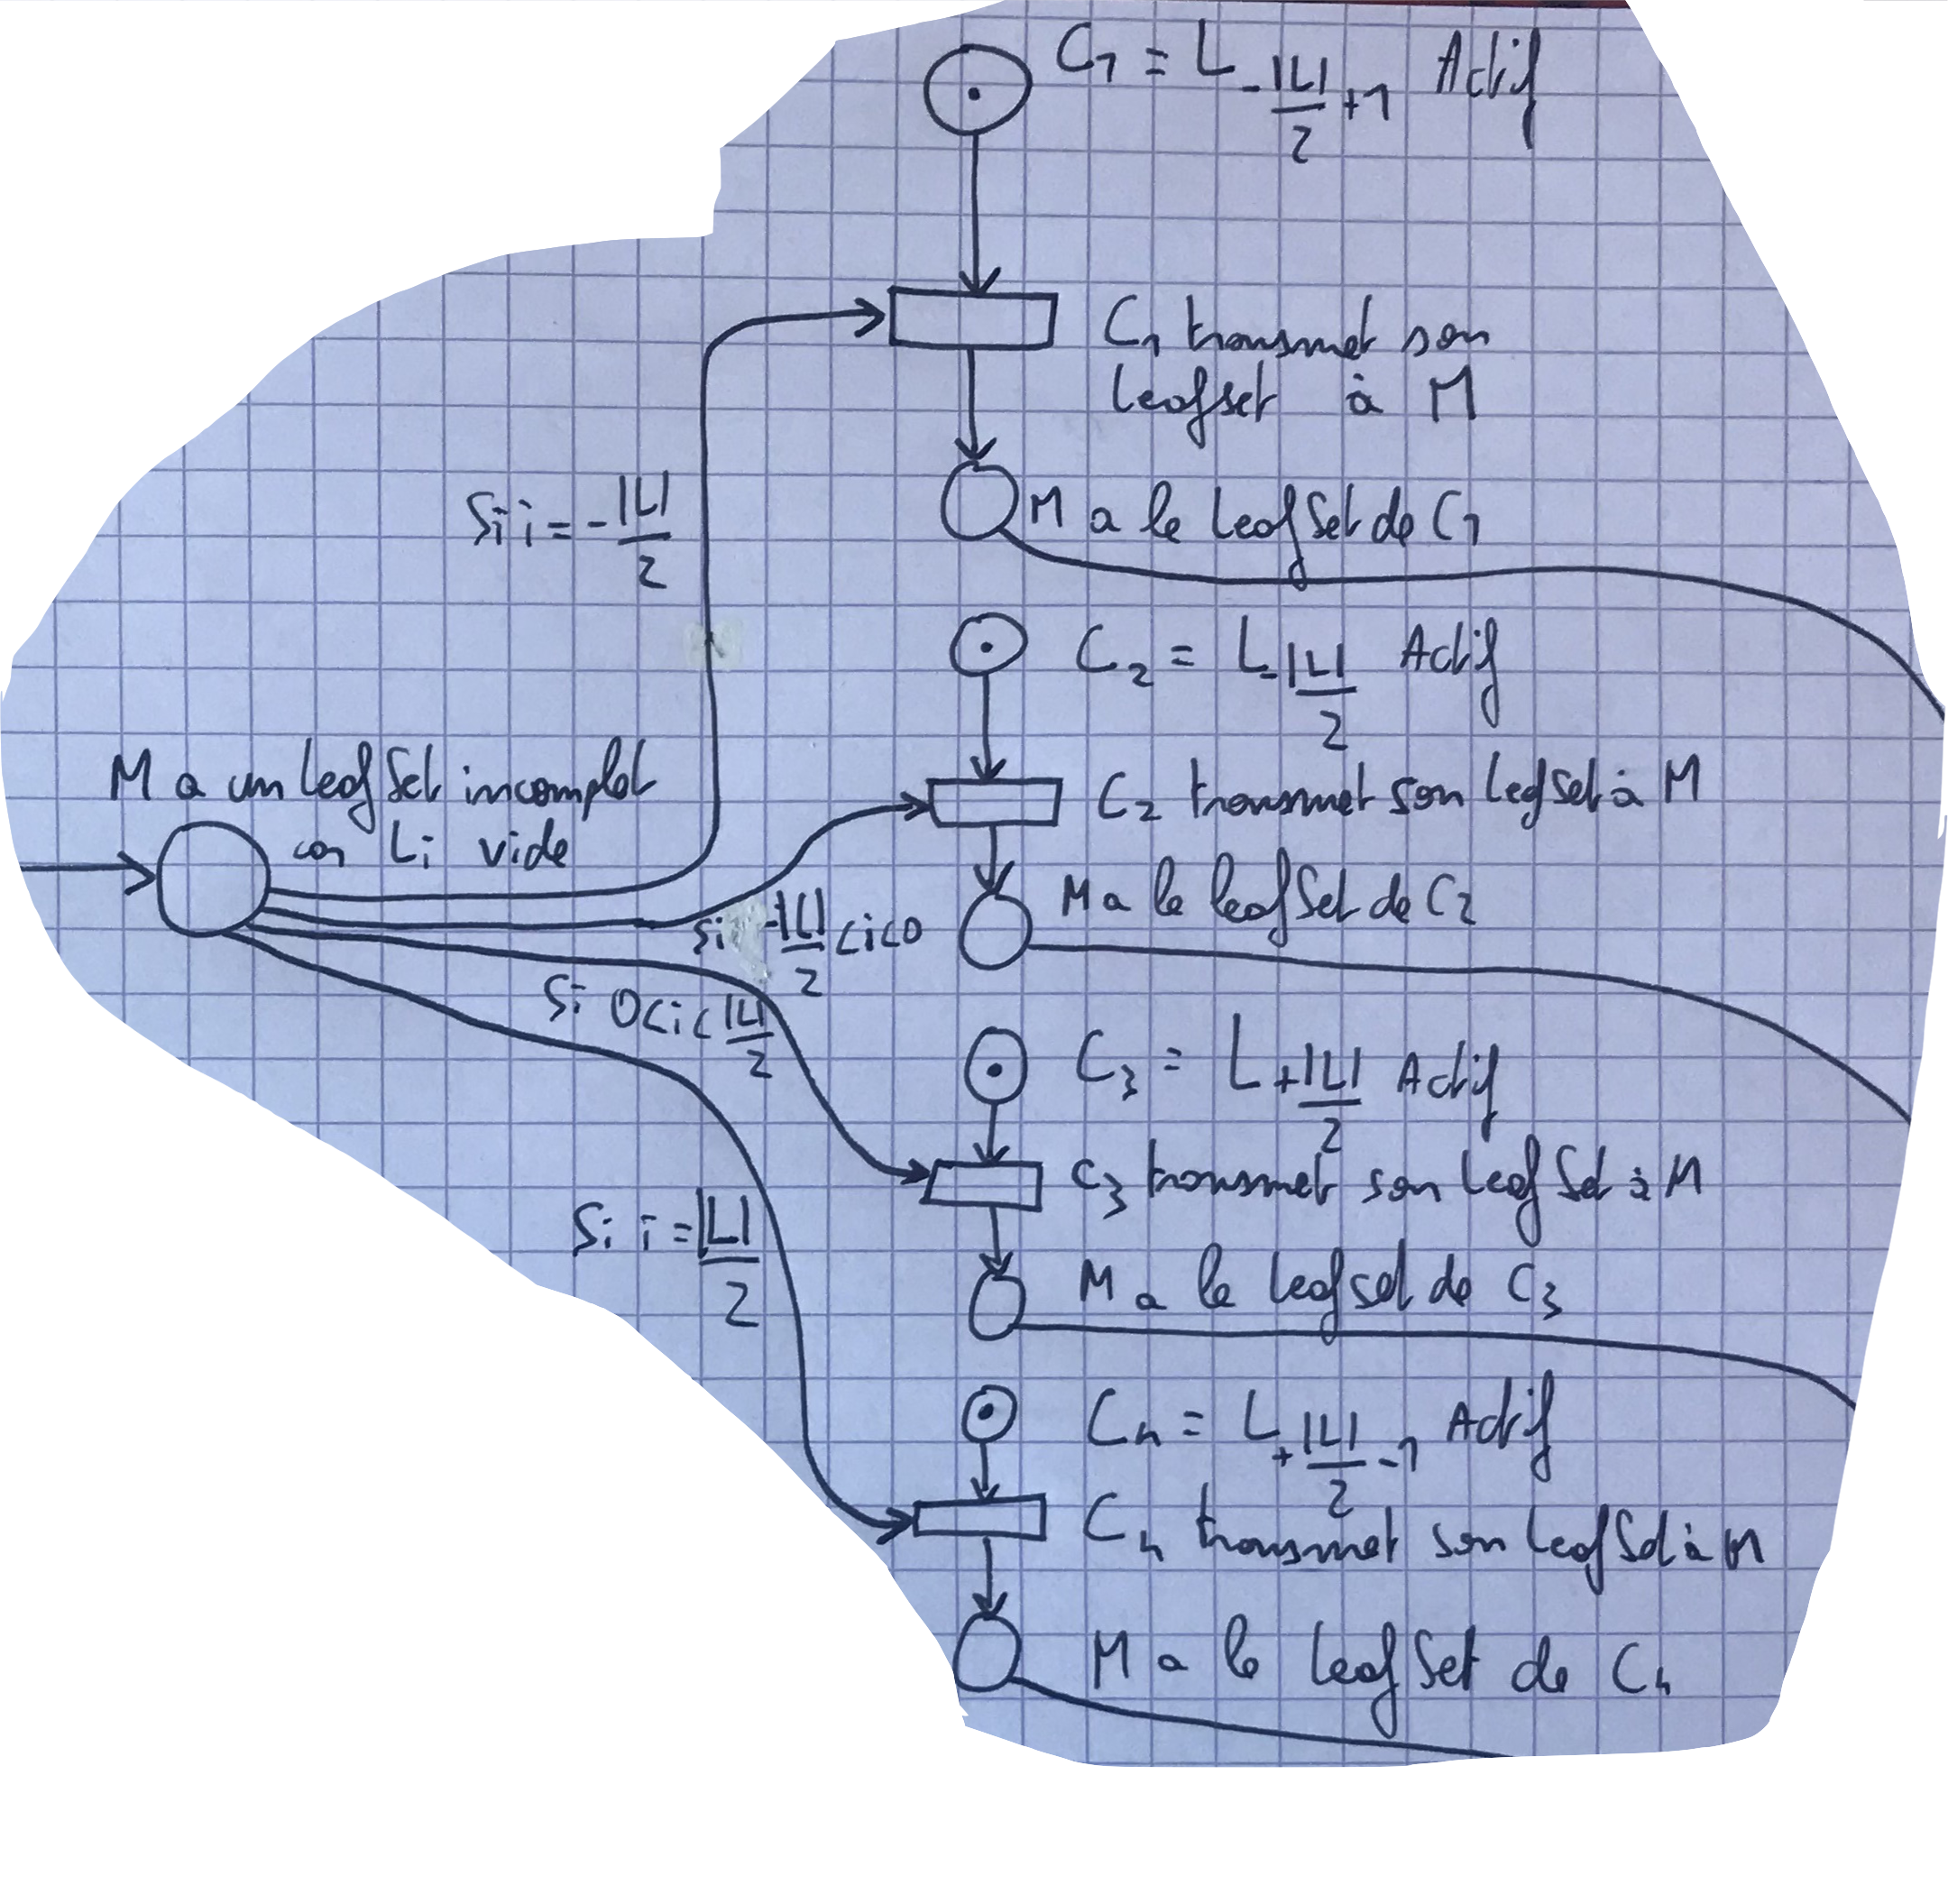
\includegraphics[scale=0.11]{partie2.png}
 \end{frame}
 \begin{frame}{LeafSet d'un réseau de Pastry}
 \includegraphics[scale=0.08]{partie3.png}
 \end{frame}
\begin{frame}{LeafSet d'un réseau de Pastry}
 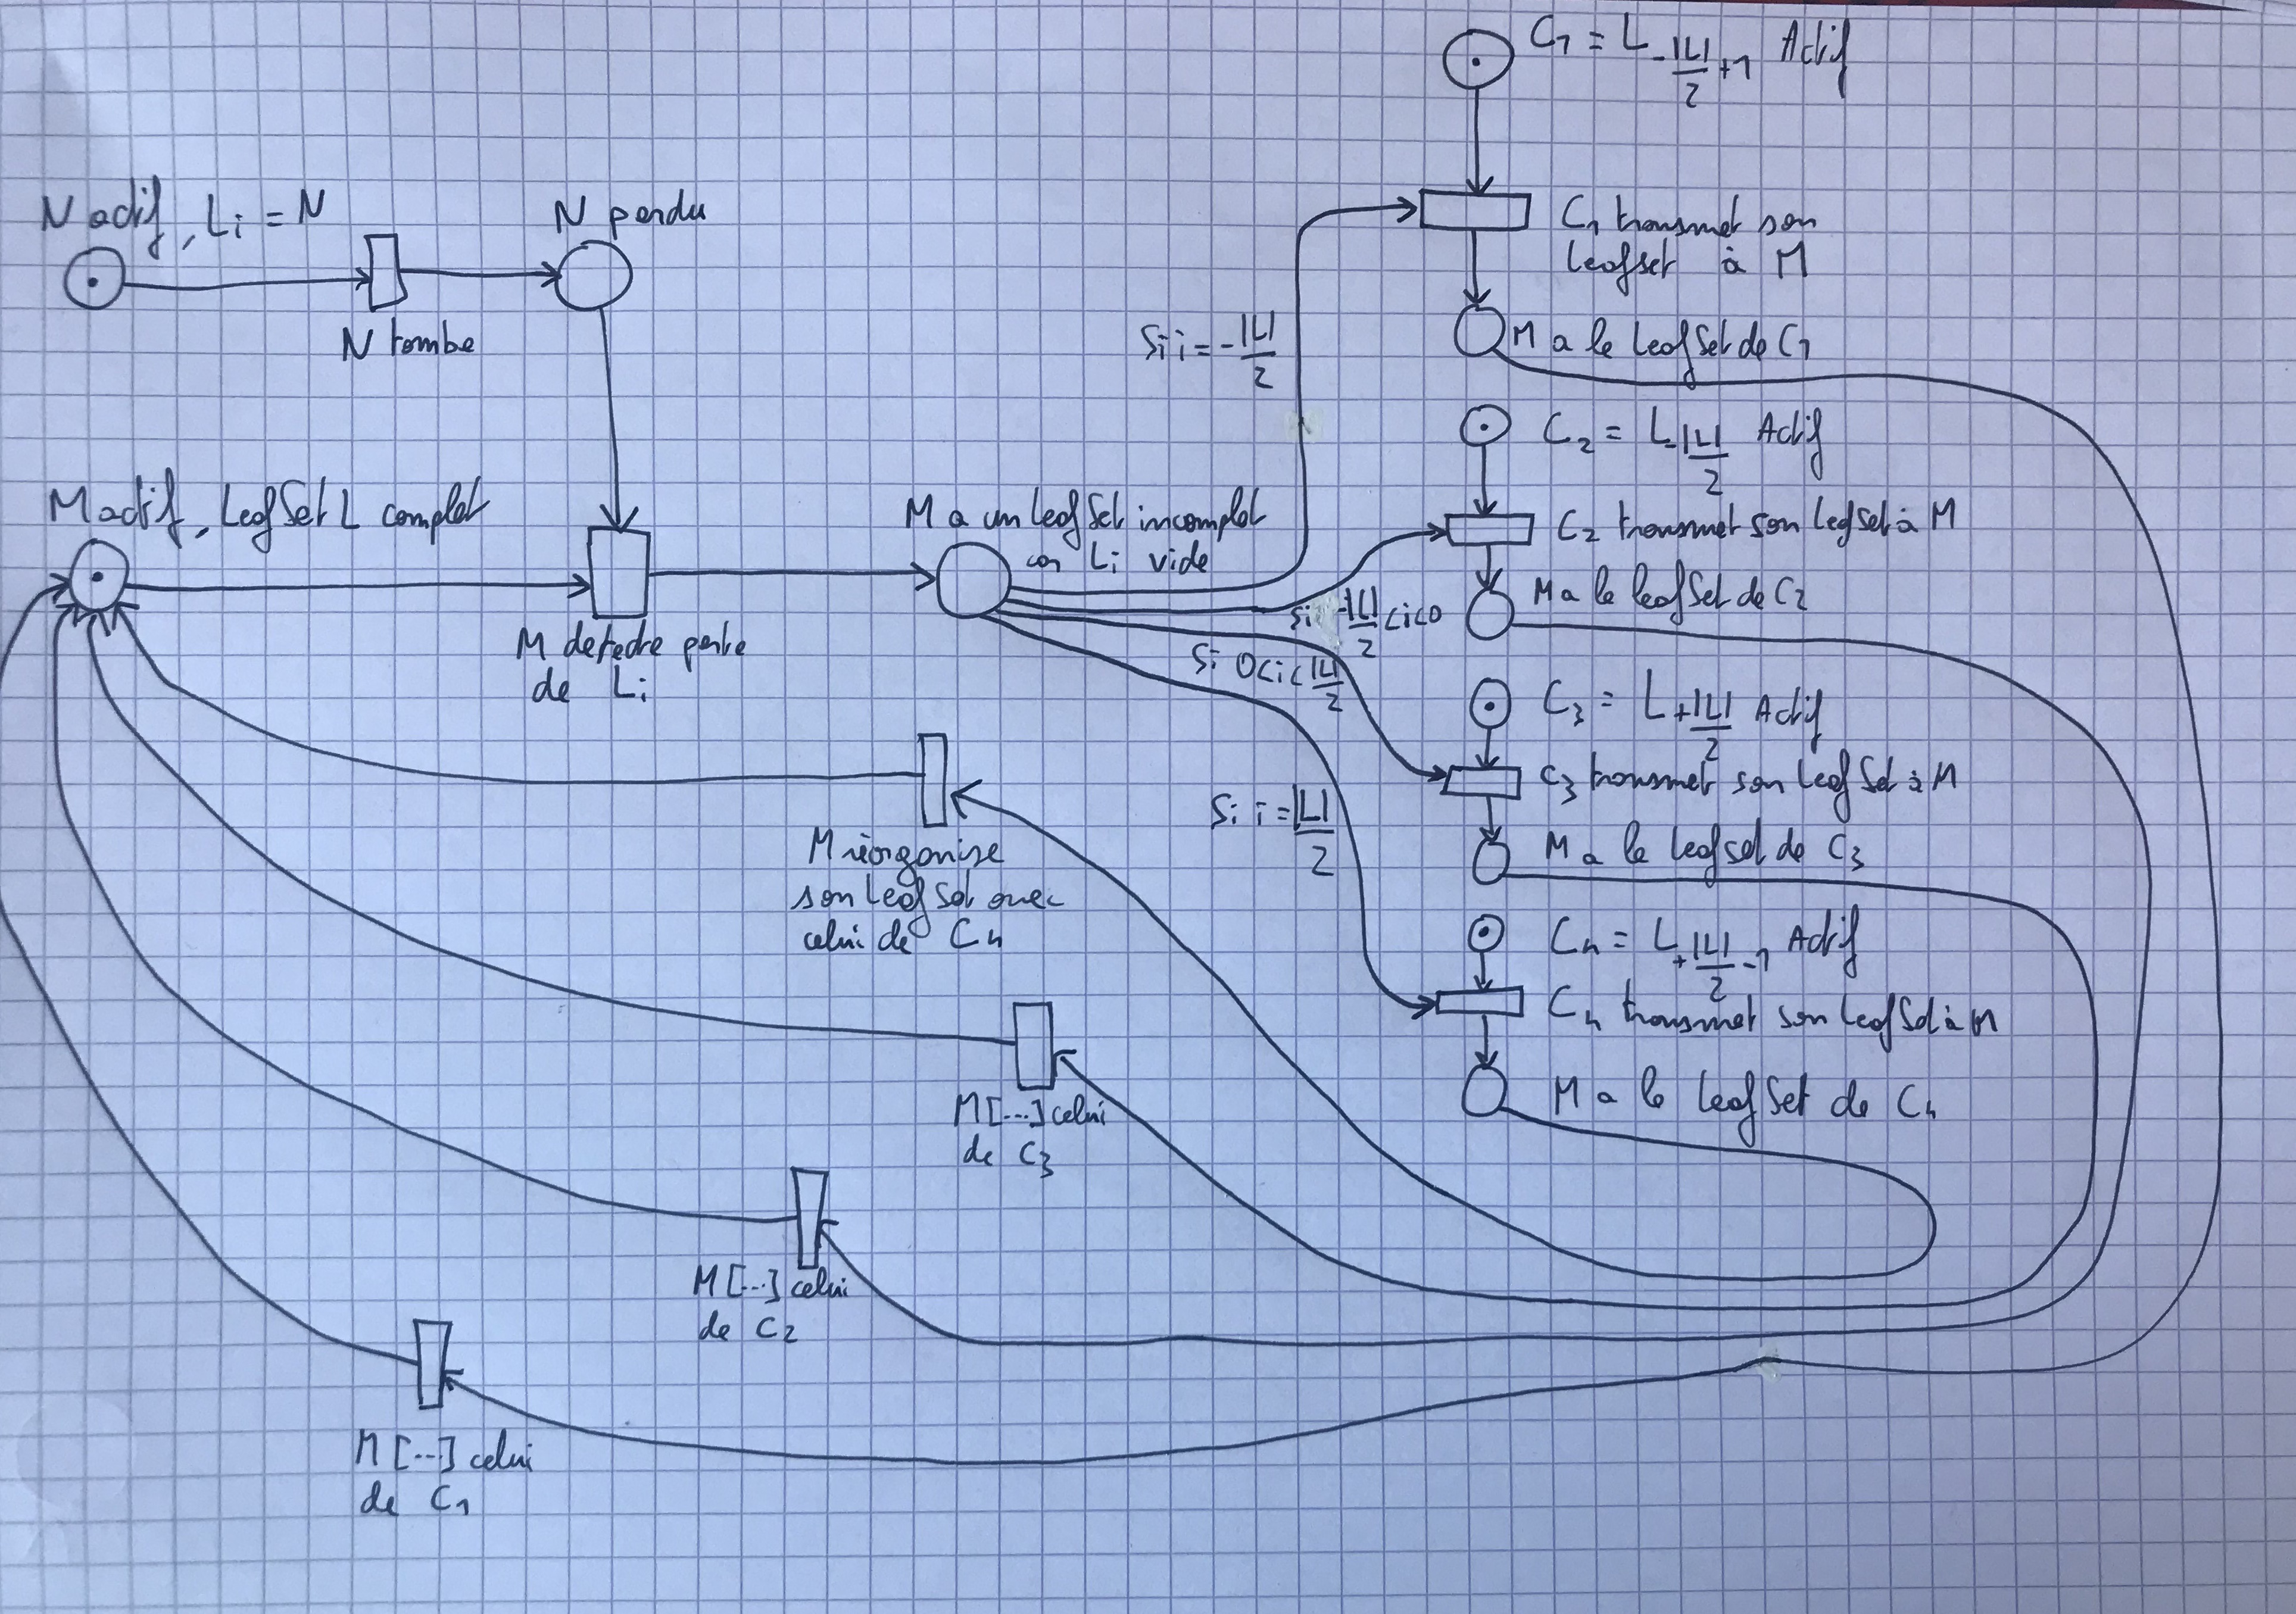
\includegraphics[scale=0.08]{petri_leafset.jpg}
 \end{frame}
 \section{Plan de la présentation du 15 Mars}
 \begin{frame}{Plan de la présentation du 15 Mars}
 
 \visible<1,2,3,4>{
 \textbf{Introduction\\I/Présentation des notions élémentaires du projet}\\
 1.Les DHT\\
 2.Les réseaux de Petri\\
 }
\visible<2,3,4>{\textbf{II/Présentation des algorithmes des systèmes répartis}\\
1. Algorithmes dans le réseau de Pastry\\
2.Algorithmes dans le réseau CAN\\}
\visible<3,4>{\textbf{ III/Modélisation des algorithmes en réseau de Petri}\\
1. Modélisation des algorithmes dans le réseau de Pastry\\
2. Modélisation des algorithmes dans le réseau CAN\\
3.Modélisation en fonction des paramètres d'entrée\\}
\visible<4>{\textbf{Conclusion}}
\end{frame}
\end{document}